%%%%%%%%%%%%%%%%%%%%%%%%%%%%%%%%%%%%%%%%%%%%%%%%%%%%%%%%%%%
% --------------------------------------------------------
% Tau
% LaTeX Template
% Version 2.4.3 (01/09/2024)
%
% Author: 
% Guillermo Jimenez (memo.notess1@gmail.com)
% 
% License:
% Creative Commons CC BY 4.0
% --------------------------------------------------------
%%%%%%%%%%%%%%%%%%%%%%%%%%%%%%%%%%%%%%%%%%%%%%%%%%%%%%%%%%%

\documentclass[9pt,a4paper,twoside]{tau-class/tau}
\usepackage[catalan]{babel}

%----------------------------------------------------------
% TITLE
%----------------------------------------------------------

\journalname{Aprenentatge Computacional}
%% TODO: Optional, you can set a fancier title if you like
\title{Classificació tiroidisme}

%----------------------------------------------------------
% AUTHORS, AFFILIATIONS AND PROFESSOR
%----------------------------------------------------------

%% TODO: Set your names here
\author[a,1]{Lluís Panal}

%----------------------------------------------------------

\affil[a]{1668072}

%----------------------------------------------------------
% FOOTER INFORMATION
%----------------------------------------------------------

\institution{Universitat Autònoma de Barcelona}
\footinfo{Class Project}
\theday{Decembre 11, 2024}
\leadauthor{Group XX} 		%% TODO: Set your group ID here
\course{Aprenentatge Computacional}

%----------------------------------------------------------
% ABSTRACT AND KEYWORDS
%----------------------------------------------------------

\begin{abstract}    
	%% TODO: Change this default abstract into something nice that describes your work.
	%% Keep it below 300 words.
    Aquest treball es centra en el desenvolupament d'un model d'aprenentatge computacional per a la classificació multiclasse de pacients amb trastorns tiroïdals. L'objectiu principal és predir l'estat de salut d'un pacient en tres categories: sa, amb hipotiroidisme o amb hipertiroidisme, a partir de característiques clíniques i analítiques disponibles. S'analitza diferents maneres de tractar la falta de dades en alguns pacients. El model es basa en tècniques d'aprenentatge supervisat, utilitzant un conjunt de dades amb múltiples variables, com resultats de proves hormonals. S'ha aplicat un conjunt de mètodes de classificació, com Decision Trees o Random Forest, avaluant el rendiment mitjançant la mètrica del f1score. Els resultats obtinguts mostren que el model és capaç de distingir de manera efectiva entre les diferents classes, proporcionant una eina útil per al diagnòstic precoç i la monitorització dels trastorns tiroïdals. \end{abstract}

%----------------------------------------------------------

%% TODO: Set appropriate keywords for your report.
\keywords{a, b, c, d}

%----------------------------------------------------------

\begin{document}
	%% Do NOT change any of this. Line numbers should be kept.
    \maketitle 
    \thispagestyle{firststyle} \tauabstract 
    \tableofcontents
    \linenumbers 
    
%----------------------------------------------------------

\section{Introduction}

    \taustart{E}ls trastorns tiroïdals, com l'hipotiroidisme i l'hipertiroidisme, són condicions mèdiques comunes que afecten un gran nombre de persones a tot el món. Aquests trastorns poden tenir un impacte significatiu en la salut general d'una persona, ja que alteren el funcionament de la glàndula tiroïdal, responsable de regular el metabolisme mitjançant les hormones tiroïdals. El diagnòstic precoç d'aquests trastorns és fonamental per a la prevenció de complicacions greus i per a un tractament adequat. No obstant això, la identificació i classificació de pacients amb trastorns tiroïdals encara pot resultar complexa a causa de la variabilitat dels símptomes i la necessitat d'anàlisis laboratorials detallades.

    L'aprenentatge computacional pot ajudar a detectar de manera automàtica la presència d'aquests trastorns. Així doncs, aquest treball explora l'aplicació d'algoritmes d'aprenentatge supervisat per a la classificació multiclasse de pacients, amb l'objectiu de desenvolupar un model capaç de diferenciar entre els pacients sans i els que tenen alguna alteració de la glàndula tiroïdal.

\section{Exploratory data analysis}
    Les dades han sigut obtingudes a través del \href{https://www.kaggle.com/datasets/emmanuelfwerr/thyroid-disease-data/data}{kaggle}.

    El dataset conté 9172 observacions i cadascuna té 31 atributs, dels quals n'hi ha 20 que són booleans, 8 que són numèrics i 3 que són categòriques (una és el sexe, que es pot passar a binària facilment). 
    
    La variable target és una de les de tipus string. Pot pendre els diferents valors: 
    '-', 'S', 'F', 'AK', 'R', 'I', 'M', 'N', 'G', 'K', 'A', 'KJ', 'L', 'MK', 'Q', 'J','C|I', 'O', 'LJ', 'H|K', 'D', 'GK', 'MI', 'P', 'FK', 'B', 'GI', 'C', 'GKJ', 'OI', 'D|R', 'E'

    La informació del dataset ens indica que si pren $'A', 'B', 'C', 'D'$ el pacient té hipertiroidisme i si pren $'E', 'F', 'G', 'H'$ té hipotiroidisme. Els altres valors indiquen o bé que està sa o bé té diagnosticat altres coses que no tenen a veure amb el tiroidisme. He assignat un 0 si el pacient té hipotiroidisme, un 1 si està sa i un 2 si té hipertiroidisme.
    
    Hi ha una variable que és única per pacient i no aporta informació, pacient\_id, que serà eliminada.

    Les dades contenen NaNs en 7 variables diferents: sex, TSH, T3, TT4, T4U, FTI i TBG. Les 6 últimes de la llista, que indiquen els nivells de diferents hormones, tenen relació amb una altra variable (cadascuna en té una de diferent), que diu si s'ha mesurat o no. Si indica que no s'ha mesurat, la variable que analitzem té un NaN. Més endavant veurem dues maneres de tractar-los.

    La figura 1 mostra la correlació entre variables que no són les mesures de les hormones ni la indicació de si s'ha mesurat o no. També s'ha eliminat les files on la variable sexe té un NaN, un 3.3\% de les dades. Es pot apreciar que la variable target no té massa correlació amb la resta de variables, la qual cosa no és massa bo. Veurem si té més correlació amb les variables eliminades per a fer la matriu.

    La figura 2 ens mostra com es distribueix els diagnòstic ens funció de l'edat i el sexe. A simple vista no es veu que tingui cap mena de relació.

    La figura 3 ens mostra les distribucions dels diagnòstics en funció de la font de referència. Aquesta gràfica sí que és més interessant, ja que hi ha dues fonts que mai diagnostiquen com a hipertiroidisme, i una, 'WEST', d'aquestes dues tampoc ho fa amb el hipotiroidisme, és a dir, diu que tothom està sa. Això passa en part perquè només hi ha 3 dades amb aquesta font.

\section{Preprocessing}

    Abans que res, vull destacar que no normalitzaré perquè al haver-hi dades mèdiques no vull perdre el seu significat.

    A continuació explicaré com he tractat diferents problemes que portaven algunes de les variables.
    \subsection{'age'}
    D'aquesta en principi sembla tot correcte ja que no hi ha NaNs ni valors negatius, però si mirem les dades que prenen el valor màxim veiem que hi ha quatre mostres que tenen molt més de 100 anys. No sé si és que no se sabia l'edat o un error humà al agafar la dada, així que com que només eren 4 mostres les he eliminat.

    \subsection{'referral\_source'}
    Aquí més que un problema és que s'ha hagut de passar de categòrica a numèrica. Per a fer-ho he creat tantes variables binàries com opcions n'hi ha, 5. D'aquestes he eliminat la que menys n'hi ha, 'WEST', ja que la informació es pot obtenir de les altres variables.

    \subsection{'sex'}
    Aquí sí que hi ha un problema: els NaNs. La variable té un 3,3\% de NaNs. Només hi ha una manera que ens permeti omplir algunes files: mirar si el pacient està embarassat. Malauradament això només omple 4 files. Com que és només un 3\% i la distribució no s'altera notablement, he decidit eliminar les files.

    \subsection{Nivells hormonals}
    Com he comentat anteriorment, per a cada indicador hi ha dues variables: una que indica si s'ha mesurat o no i l'altres que dona la mesura si l'altre és positiva o té un NaN si l'altre és negativa. No hi ha cap NaN que en files on sí que s'hagi mesurat, per això he eliminat les columnes que indiquen si s'ha mesurat o no. Com que si mirem totes les files que tenen un NaN en alguna de les sis columnes em quedaria sense dades, no les puc eliminar, les he d'omplir. Ho he provat de dues maneres diferents.

    \subsubsection{Canviar els Nans per -1}
    Aquesta estratègia pot arribar a ser útil en models no massa simples, no pot funcionar amb una regressió logística, per exemple, ja que intentaria predir amb aquest valor de la mateixa manera que amb qualsevol altre. Un altre problema que pot portar és que no tots els indicadors tenen la mateixa escala, és a dir, no és el mateix per un indicador que pot pendre valors entre 0 i 10 que per una altra que pot prendre valors entre 0 i 1000. L'escala de les dades també pot ser un problema per un altre motiu: al tenir escales diferents per a les variables, pot ser que afecti als paràmetres de manera que no només tinguin en compte la importància. Per això el que vaig fer va ser dividir cada indicador per el valor màxim que està considerat com a sa, d'aquesta manera tot quedava a escales similars. A més a més, el -1 ara és prou petit (gran negativament) com per a separar-se de les mostres.

    Ara només l'edat pren nombres molt grans en comparació a la resta. Com que només hi ha edats entre 1 i 100 anys, la vaig dividir entre 100 per a tenir-les amb un rang entre 0 i 1 a una escala similar a les altres variables.

    \subsubsection{Discretitzar els indicadors}
    La segona opció va ser separar els valors en intervals, de manera que si hi havia una mesura feta la fila tindria un 1 en un dels intervals i un 0 en els altres, i si, en canvi, hi hagués un NaN, tots els intervals tindrien un 0. La opció final que he triat ha sigut fer 3 intervals, un pels que tenen un valor baix, un pels que tenen un valor normal i un últim pels que tenen un valor alt. Els llindars per a determinar a cada interval pertany cada pacient els he buscat. He trobat els següents:
    TODO: posar intervals

    Vull destacar que també vaig provar de separar-ho en 6 intervals, separar cadascun dels 3 anteriors en dos. Els resultats obtinguts eren lleugerament inferiors, així que ho vaig descartar. Una de les causes podria ser que aquests nous llindars els vaig posar de manera arbitrària, ja que no hi havia cap criteri oficial.

    Amb aquesta manera de tenir en compte els NaNs, l'única variable que ara no és binària és l'edat. Així doncs, també la vaig discretitzar en 6 intervals. Ara doncs, totes les variables són binàries
    

    \LaTeX is based on the idea of defining commands (or macros) that control the presentation of the text on a document. As a matter of fact, \LaTeX ignores whitespace except for double newlines (pressing intro twice), which is used to delimit paragraphs. Commands are usually preceeded by a backslash (\\) and have a number of arguments, if any, between braces (\{ and \}). You can set a \textbf{bold} or an \textit{italic} typeface using the \verb|\textbf{.}| and \verb|\textit{.}| commands. You can also {\tiny change the size of the font for a scope}. You can change {\color{red} text color} using the \verb|\color{col}| command. 

    Nevertheless, you should mostly refrain from formatting text explicitly. \LaTeX provides commands for recurring types of  text modifications with some batteries included. For instance, if you want to divide your text in chunks under prominent titles you can use the \verb|\section{.}|, \verb|\subsection{.}|, \verb|\subsubsection{.}| ... etc commands, which will handle everything for you. These titles will automatically appear in the table of contents, they will be properly numbered in the order of appearance, etc. If you are writing a book, you can also use the \verb|\part{.}| and \verb|\chapter{.}| commands for this.

    Many \LaTeX constructs are built around the \verb|\begin{environment}| and \verb|\end{environment}| commands. You write some text between these two commands that is to be formatted according to the rules of the given environment. With this, you can write

    \begin{itemize}
        \item Bullet point lists (environment itemize)
    \end{itemize}

    \begin{enumerate}
        \item Enumerations (environment enumerate)
    \end{enumerate}

    \begin{info}
        ... or some custom stuff as well. The possibilities are quite endless, really.
    \end{info}

    You can edit \LaTeX in any text editor of your choice. I suggest that you try \href{https://www.overleaf.com/}{Overleaf} first, because the editing experience is very simple and very close to that of a shared Google Docs. These days they have gotten quite stingy however, so I suggest using VS Code with the \LaTeX Workshop extension instead. If you need to share the document, just put it in a Git repository. There are a myriad alternatives, so go out there and try what works for you.
		
\section{Figures and tables} \label{sec:table}

    \subsection{Figures}
		
	Fig. \ref{fig:figure} shows an example figure. Figures can be referenced using \verb|\ref{ident}|, where \texttt{name} is a previously-defined \verb|\label{name}| for any object in the document. You can actually also do this with sections (Section \ref{sec:table}) or equations or other types of objects that will be seen below.
		
	\begin{figure}[H]
		\centering
		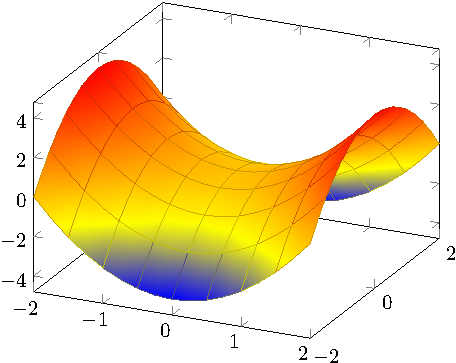
\includegraphics[width=0.75\columnwidth]{Example.pdf}
		\caption{Example figure obtained from PGFPlots \cite{PFGPlots}.}
		\label{fig:figure}
	\end{figure}
		
        Fig. \ref{fig:examplefloat} shows an example of two figures that cover the width of the page. It can be placed at the top or bottom of the page. The space between the figures can also be changed using the \verb|\hspace{Xpt}| command.
		
        \begin{figure*}[tp] % t for position at the top of the current page; b for position at the bottom; p for new page
		\centering
		  \begin{subfigure}[b]{0.38\linewidth} % Fig (a)
			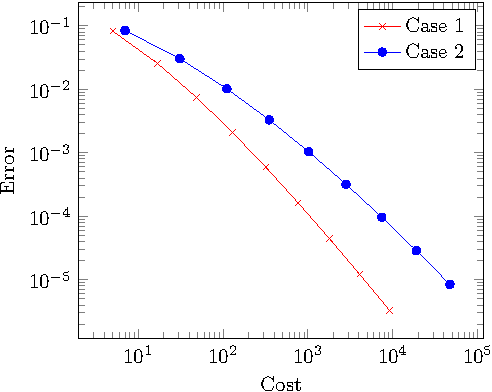
\includegraphics[width=\linewidth]{Example2.pdf}
			\caption{Example left figure.}
			\label{fig:figa}
		\end{subfigure}
			\hspace{20pt}   % Space between the figures
		\begin{subfigure}[b]{0.375\linewidth} % Fig (b)
			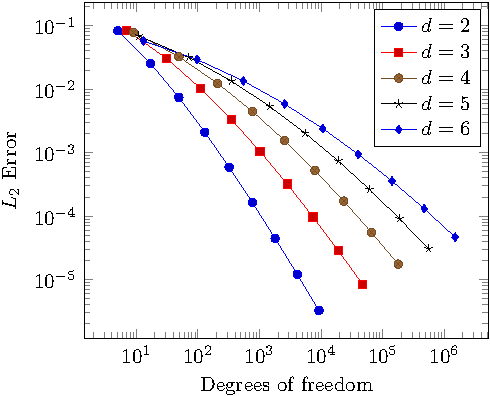
\includegraphics[width=\linewidth]{Example3.pdf}
			\caption{Example right figure.}
			\label{fig:figb}
		\end{subfigure}
		\caption{Example figure that covers the width of the page obtained from PGFPlots \cite{PFGPlots}.}
		\label{fig:examplefloat}
	\end{figure*}

    \begin{info}
    	Figures in \LaTeX are known to be quite anarchic. You should always wait until the very end to place them well into the document. In any case, you should always reference the Figure and provide a Caption so that it can be contextualised even when it lies far away from the text that accompanies it.
    \end{info}

    \begin{info}
    	Avoid raster graphics (jpeg, png) for figures if you can. Always use vectorial formats for plots and diagrams. The preferred formats for vectorial images are SVGs converted to Encapsulated Post-Script (.eps, you can use Inkscape to perform this conversion) or PDF files. Regardless of the image format you are using, generate reasonably high-resolution files (the usual is 300dpi, which means 300 pixels per squared inch). \textbf{Keep in mind that Matplotlib can be configured to generate plots with these settings.}
    \end{info}

    \subsection{Tables}
	
        Table \ref{tab:table} shows an example table. The \verb|\tabletext{}| is used to add notes to tables easily. 

        \begin{info}
        	This template uses the \texttt{booktabs} package by default. This package makes typesetting nice tables easier, but it imposes some general design guidelines. The most prominent is the distinction between middle and edge rules (horizontal lines) and the discouragement of vertical lines.
        \end{info}

        \begin{info}
        	You should \textbf{always} avoid typesetting tables by hand. Use tools such as \href{https://www.tablesgenerator.com/}{this one} to spare yourself some unnecessary pain.
        \end{info}
		
	\begin{table}[H]
		\centering
		\caption{Small example table.}
		\label{tab:table}
		\begin{tabular}{cc}
			\toprule
			\textbf{Column 1} & \textbf{Column 2} \\
			\midrule
			Data 1 & Data 2 \\
			Data 3 & Data 4 \\
			\bottomrule
		\end{tabular}
			
            \tabletext{Note: I'm a table text for additional information.}
			
	\end{table}
		
\section{Tau packages}

    \subsection{Tauenvs}
	
        This template has its own environment package \textit{tauenvs.sty} designed to enhance the presentation of the document. Among these custom environments are \textit{tauenv}, \textit{info} and \textit{note}.
		
        There are two environments which have a predefined title. These can be included by the command \verb|\begin{note}| and \verb|\begin{info}|. All the environments have the same style.
			
        An example using the tau environment is shown below.
		
	\begin{tauenv}[frametitle=Environment with custom title]
            This is an example of the custom title environment. To add a title type \verb|[frametitle=Your title]| next to the beginning of the environment (as shown in this example).
	\end{tauenv}
		
        Tauenv is the only environment that you can customize its title. On the other hand, info and note adapt their title to Spanish automatically when this language package is defined.
		
    \subsection{Taubabel}

        In this new version, we have included a package called \textit{taubabel}, which have all the commands that automatically translate from English to Spanish when this language package is defined. 
        
        By default, tau displays its content in English. However, at the beginning of the document you will find a recommendation when writing in Spanish. 
		
        \textit{Note:} You may modify this package if you want to use other language than English or Spanish. This will make easier to translate the document without having to modify the class document.
		
\section{Equation}

    Equation \ref{ec:equation}, shows the Schrödinger equation as an example. 
	\begin{equation} \label{ec:equation}
		\frac{\hbar^2}{2m}\nabla^2\Psi + V(\mathbf{r})\Psi = -i\hbar \frac{\partial\Psi}{\partial t}
	\end{equation} 
    The \textit{amssymb} package was not necessary to include, because stix2 font incorporates mathematical symbols for writing quality equations. In case you choose another font, uncomment this package in tau-class/tau.cls/math packages.
	
    If you want to change the values that adjust the spacing above and below the equations, play with \verb|\setlength{\eqskip}{8pt}| value until the preferred spacing is set.
	
\section{Adding codes}
	
    This class\footnote{Hello there! I am a footnote :)} includes the \textit{listings} package, which offers customized features for adding codes in \LaTeX\ documents specifically for C, C++, \LaTeX\ and Matlab. 
	
    You can customize the format in tau-class/tau.cls/listings style.
	
        \nolinenumbers
            \lstinputlisting[caption=Example of Matlab code., language=Matlab,label=code]{example.m}
	\linenumbers
	
    If line numbering is defined at the beginning of the document, I recommend placing the command \verb|\nolinenumbers| at the start and \verb|\linenumbers| at the end of the code. 
	
    This will temporarily remove line numbering and the code will look better as shown in Code \ref{code}.
	
\section{References}

    The default formatting for references follows the IEEE style. You can modify the style of your references, for that, go to tau-class/tau.cls/biblatex. See appendix for more information.
	
\section{Appendix}

    \subsection{Alternative title}

        You can make the following modification in tau-class/tau.cls/title preferences section to change the position of the title.

\nolinenumbers
\begin{lstlisting}[language=TeX, caption=Alternative title.]
\newcommand{\titlepos}{\centering}
\end{lstlisting}
\linenumbers

	This will move the title to the center. 

    \subsection{Info environment}

        An example of the info environment declared in the ‘tauenvs.sty’ package is shown below. Remember that \textit{info} and \textit{note} are the only packages that translate their title (English or Spanish).
		
	\begin{info}
		Small example of info environment.
	\end{info}

    \subsection{Equation skip value}

        With the \verb|\eqskip| command you can change the spacing for equations. The default \textit{eqskip} value is 8pt.

\nolinenumbers
\begin{lstlisting}[language=TeX, caption=Equation skip code.]
\newlength{\eqskip}\setlength{\eqskip}{8pt}
	\expandafter\def\expandafter\normalsize\expandafter{%
		\normalsize%
		\setlength\abovedisplayskip{\eqskip}%
		\setlength\belowdisplayskip{\eqskip}%
		\setlength\abovedisplayshortskip{\eqskip-\baselineskip}%
		\setlength\belowdisplayshortskip{\eqskip}%
	}
\end{lstlisting}
\linenumbers
		
    \subsection{References}
		
        In case you require another reference style, you can go to tau-class/tau.cls/biblatex and modify the following.
		
\nolinenumbers
\begin{lstlisting}[language=TeX, caption=References style.]
\RequirePackage[
	backend=biber,
	style=ieee,
	sorting=ynt
]{biblatex}
\end{lstlisting}
\linenumbers

        By default, \textit{tau class} has its own .bib for this example, if you want to name your own bib file, change the \textit{addbibresource}.
		
\nolinenumbers
\begin{lstlisting}[language=TeX]
\addbibresource{tau.bib}
\end{lstlisting}
\linenumbers

\section{Acknowledgements}

Tau \LaTeX template built by Guillermo Jimenez.

%----------------------------------------------------------

\addcontentsline{toc}{section}{References}
\printbibliography

%----------------------------------------------------------

\end{document}